\section{算法}


\subsection{算法的表示方法}

\begin{frame}
    \frametitle{算法的表示方法}
    一个问题可以设计不同的算法来求解，而同一个算法可以采用不同的形式来表述，常用的描述方法有以下几种：
    \begin{itemize}
      \item 自然语言
      \item 传统流程图
      \item 伪代码（类语言）
      \item 高级程序语言
    \end{itemize}
\end{frame}

\begin{frame}
    \frametitle{自然语言}
    自然语言表示算法就是把算法的各个步骤，依次用人们熟悉的自然语言表示出来。日常生活中使用自然语言，通俗易懂，容易掌握，但是语句繁琐、文字冗长，很难清楚表达算法的逻辑流程，不严谨，容易出现“歧义性”，因此，自然语言通常用于介绍算法的概要思路。
    
    \smallskip
    \begin{quote}
      “去市场买一个西瓜，如果看到西红柿，就买两个”
    \end{quote}

    \begin{block}{用自然语言描述：输入x、y，计算z=x÷y，输出z。}     

      （1）输入变量x，y；

      （2）判断y是否为0；

      （3）如果y=0，则输出出错提示信息；

      （4）否则计算z=x/y；

      （5）输出z。
    \end{block}
\end{frame}


\begin{frame}
    \frametitle{传统流程图}
    流程图是描述算法的常用工具，是采用美国国家标准化协会规定的一组图形符号及文字说明来描述计算过程的图形。流程图直观地表示了算法的整个结构，易于理解，便于检查修改，但不方便表达数据处理过程。

        \begin{minipage}{0.48\linewidth}
            \begin{figure}[h]
                \centering
                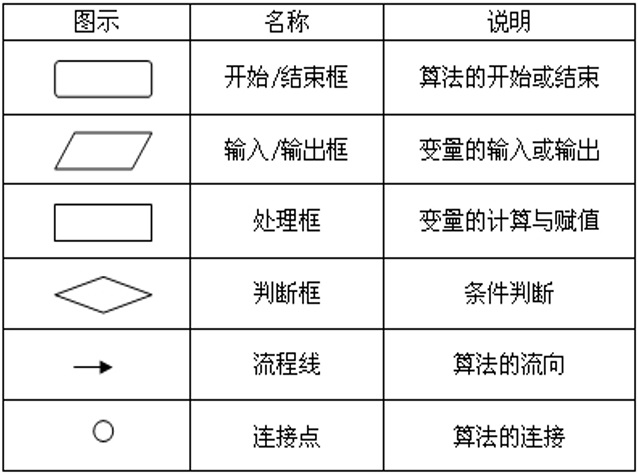
\includegraphics[width=\linewidth]{images/flow_chart1.jpg}
              \end{figure}
        \end{minipage}\hfill
        \begin{minipage}{0.48\linewidth}
            \begin{block}{输入x、y，计算z=x÷y，输出z。}  
                \hspace{1.5cm} \begin{tikzpicture}[semithick,node distance=1.5cm,scale=0.48,every node/.style={scale=0.48}]
                  \node (start) [startstop] {开始};
                  \node (in) [io, below of=start] {输入$x,y$};
                  \node (choice) [decision, below of=in] {$y=0?$};
                  \node (pro1) [op, below of=choice,xshift=-2cm] {错误提示};
                  \node (pro2) [op, below of=choice,xshift=2cm] {$z=x/y$};
                  \node (out) [io, below of=pro2] {输出$z$};
                  \node (end) [startstop, below of=out,xshift=-2cm] {结束};
                  \draw [->] (start) -- (in);
                  \draw [->] (in) -- (choice);
                  \draw [->] (choice) -| node [above] {Yes} (pro1);
                  \draw [->] (choice) -| node [above] {No} (pro2);
                  \draw [->] (pro2) -- (out);
                  \draw [->] (out) -- ++ (0,-0.7) -| (end);
                  \draw [->] (pro1) -- ++ (0,-2.2) -| (end);
              \end{tikzpicture}
              \end{block} 
        \end{minipage}
 
\end{frame}

\begin{frame}
    \frametitle{常用的制作流程图的软件}
    \begin{itemize}
      \item {\cbf{Visio}}
      
      微软推出的一款流程图制作工具，内置大量的模板方便使用，界面简洁操作方便，功能全面。
      
      \item {\cbf{Word/PowerPoint}}
      
      可以做基本的流程图，容易上手。
      
      \item {\cbf{网页版在线作图工具}}
        \begin{itemize}
          \item Processon \link{https://www.processon.com}
          \item draw.io \link{https://app.diagrams.net/}
        \end{itemize}
    \end{itemize}
\end{frame}

\begin{frame}
    \frametitle{伪代码}
    伪代码也称类语言，接近于高级语言但又不是严格意义上的高级语言，是一种介于自然语言与计算机语言之间的算法描述方式。伪代码具有高级语言的一般语句结构，撇掉语言中的细节，以便把注意力主要集中在算法处理步骤本身的描述上。
    % 伪代码是一种接近自然语言的算法描述形式，其目的是在不涉及具体实现（各种编程语言）的情况下将算法的流程和含义清楚的表达出来，因此它没有一个统一的规范，有的仅仅是在长期的实践过程中形成的一些约定俗成的表达样式。
    % 赋值操作一般使用左箭头「<—」表示。
    \vspace{-4pt}
      \begin{algorithm}[H]  
        \caption{Calculate $y = x/y$}
      \begin{algorithmic}[1]
        \Begin
        \State \textbf{input} $x,y$;
        \If {$y=0$}
        \State \textbf{print} “Error!”;
        \Else
        \State $z \gets x/y$
        \State \textbf{return}($z$);
        \End
        \end{algorithmic}
        \end{algorithm}
\end{frame}

\begin{frame}[fragile]
    \frametitle{高级程序语言}
    高级程序语言就是用计算机程序设计语言直接表达算法，是可以在计算机上直接运行的源程序。高级程序语言描述的算法具有严格、准确的优点，但也有语言细节过多的弱点。

\begin{codeblock}{用python语言描述：输入x、y，计算z=x÷y，输出z。}
  x = float(input("请输入x："))
  y = float(input("请输入y："))
  if y == 0:
      print("分母不能为0！")
  else:
      z = x/y
      print(z)
\end{codeblock}
\end{frame}



\subsection{算法的结构}


\begin{frame}
    \frametitle{算法的三种结构}
    \begin{itemize}
      \item {\cbf{顺序结构}}
      
      这种结构最简单，各个步骤是按先后顺序执行的。
      
      \item {\cbf{分支结构}}
      
      分支结构又称选择结构，用于判断给定的条件，根据判断的结果判断某些条件，根据判断的结果来控制程序的流程。
      
      \item {\cbf{循环结构}}
      
      循环结构又称为重复结构，指在程序中需要反复执行某个功能而设置的一种程序结构。它由循环体中的条件，判断继续执行某个功能还是退出循环。
       
    \end{itemize}
\end{frame}

\begin{frame}
    \frametitle{顺序结构}
    顺序结构的各个步骤是按先后顺序执行的。

      \begin{minipage}{0.48\linewidth}
            \begin{center}
              \begin{tikzpicture}[semithick,node distance=1.5cm]
                \node (pro1) [op] {步骤A};
                \node (pro2) [op, below of=pro1] {步骤B};
                \node (pro3) [op, below of=pro2] {步骤C};
                \graph[use existing nodes=true]{
                    pro1  ->  pro2  ->  pro3;
                };
                \draw[<-] (pro1) -- (0,1);
                \draw[->] (pro3) -- ++ (0,-1);
            \end{tikzpicture}
            \end{center}
        \end{minipage}\hfill
        \begin{minipage}{0.48\linewidth}
          \begin{block}{输入a和b， 输出a+b的和}
            \begin{center}
              \begin{tikzpicture}[semithick,node distance=1.5cm,scale=0.7,every node/.style={scale=0.7}]
                \node (start) [startstop] {开始};
                \node (in) [io, below of=start] {输入$a,b$};
                \node (pro) [op, below of=in] {$c = a + b$};
                \node (out) [io, below of=pro] {输出$c$};
                \node (end) [startstop, below of=out] {结束};
                \graph[use existing nodes=true]{
                start  ->  in  ->  pro  ->  out -> end ;
                };
              \end{tikzpicture}
            \end{center}
          \end{block}
        \end{minipage}
\end{frame}

\begin{frame}
  \frametitle{顺序结构}
    \begin{minipage}{0.48\linewidth}
      \begin{block}{例}交换2个变量的值， 然后输出。
      \end{block}
          \begin{center}
            \begin{tikzpicture}[semithick,node distance=2cm,scale=1.2,every node/.style={scale=1.2}]
              \node (pro1) [circle,fill=DarkSeaGreen1] {$a$};
              \node (pro2) [circle,right of=pro1, xshift=2cm,fill=DarkSeaGreen1] {$b$};
              \node (pro3) [circle,below of=pro1, xshift=2cm,fill=IndianRed1] {$t$};
              \draw[->] (pro1.south) to  [bend right=45] node [above] {1} (pro3.west);
              \draw[->] (pro3.east) to [bend right=45] node [above] {3} (pro2.south);
              \draw[->] (pro2.north) to [bend right=60] node [below] {2} (pro1.north);
          \end{tikzpicture}
          \end{center}
      \end{minipage}\hfill
      \begin{minipage}{0.48\linewidth}
          \begin{center}
            \begin{tikzpicture}[semithick,node distance=1.5cm,scale=0.7,every node/.style={scale=0.7}]
              \node (start) [startstop] {开始};
              \node (in) [io, below of=start] {输入$a,b$};
              \node (pro1) [op, below of=in] {\red{$t=a$}};
              \node (pro2) [op, below of=pro1] {\red{$a=b$}};
              \node (pro3) [op, below of=pro2] {\red{$b=t$}};
              \node (out) [io, below of=pro3] {输出$a,b$};
              \node (end) [startstop, below of=out] {结束};
              \graph[use existing nodes=true]{
              start  ->  in ->  pro1 ->  pro2 ->  pro3 ->  out -> end ;
              };
          \end{tikzpicture}
          \end{center}
      \end{minipage}
\end{frame}


\begin{frame}
    \frametitle{分支结构}
      有些操作需要满足一定的条件才能进行，在操作前需要进行条件判断。

      \smallskip
      \begin{minipage}{0.4\linewidth}
        \begin{center}
          \begin{tikzpicture}[semithick,node distance=2cm,scale=0.9,every node/.style={scale=0.9}]
            \node (start) [startstop] {开始};
            \node (choice) [decision,below of=start] {晴天？};
            \node (pro) [op,below of=choice] {洗衣};
            \node (end) [startstop,below of=pro] {结束};
            \graph[use existing nodes=true]{
                start -> choice ->["Yes"right] pro -> end ;
                };
                \draw [->] (choice)  -- ++ (-2,0)  node [above,midway] {No} -- ++ (0,-3.2) -| (end);
            \node at (-3,-3) {\cbf{单分支：}};
        \end{tikzpicture}
        \end{center}
      \end{minipage}\hfill
      \begin{minipage}{0.58\linewidth}
        \begin{center}
          \begin{tikzpicture}[semithick,node distance=2cm,scale=0.9,every node/.style={scale=0.9}]
            \node (start) [startstop] {开始};
            \node (choice) [decision,below of=start] {晴天？};
            \node (pro1) [op,below of=choice,xshift=-2cm] {洗衣};
            \node (pro2) [op,below of=choice,xshift=2cm] {擦地};
            \node (end) [startstop,below of=pro1,xshift=2cm] {结束};
            \draw [->] (start) -- (choice);
            \draw [->] (choice) -| (pro1) node [above,midway] {Yes};
            \draw [->] (choice) -| (pro2) node [above,midway] {No};
            \draw [->] (pro1) -- ++ (0,-1) -| (end) ;
            \draw [->] (pro2) -- ++ (0,-1) -| (end) ;
            \node at (-5,-3) {\cbf{双分支：}};
        \end{tikzpicture}
        \end{center}
      \end{minipage}
\end{frame}

\begin{frame}
    \frametitle{分支结构}
      \begin{minipage}{0.48\linewidth}
            \begin{block}{例}
              将a，b变量中的数据按从大到小的顺序排序，即处理后a中存放两数中的大数，b存放小者。
            \end{block}
              \begin{itemize}
                \item 如果a>b，则不需要处理；
                \item 如果a<b，则需要交换a与b的值。
              \end{itemize}            
        \end{minipage}\hfill
        \begin{minipage}{0.48\linewidth}
          \begin{center}
            \begin{tikzpicture}[semithick,node distance=1.5cm,scale=0.63,every node/.style={scale=0.63}]
              \node (start) [startstop] {开始};
              \node (in) [io, below of=start] {输入$a,b$};
              \node (choice) [decision, below of=in] {$b>a?$};
              \node (pro1) [op, below of=choice] {$t=a$};
              \node (pro2) [op, below of=pro1] {$a=b$};
              \node (pro3) [op, below of=pro2] {$b=t$};
              \node (out) [io, below of=pro3] {输出$a,b$};
              \node (end) [startstop, below of=out] {结束};
              \graph[use existing nodes=true]{
              start  ->  in -> choice -> ["Yes",right] pro1 ->  pro2 ->  pro3 ->  out -> end ;
              };
              \draw [->] (choice) -- ++ (-2.5,0) node [above] {No} -- ++ (0,-5.2) -| (out);
          \end{tikzpicture}
          \end{center}
        \end{minipage}
\end{frame}

\begin{frame}
    \frametitle{}
    \begin{block}{例}输入2个数，求最大值输出。      
    \end{block}
      \begin{minipage}{0.48\linewidth}
        \begin{center}
          \begin{tikzpicture}[semithick,node distance=1.5cm,scale=0.7,every node/.style={scale=0.7}]
            \node (start) [startstop] {开始};
            \node (in) [io, below of=start] {输入$a,b$};
            \node (choice) [decision, below of=in] {$a>b?$};
            \node (pro1) [op, below of=choice,xshift=-2cm] {$max=a$};
            \node (pro2) [op, below of=choice,xshift=2cm] {$max=b$};
            \node (out) [io, below of=pro1,xshift=2cm] {输出$max$};
            \node (end) [startstop, below of=out] {结束};
            \draw [->] (start) -- (in);
            \draw [->] (in) -- (choice);
            \draw [->] (choice) -| node [above] {Yes}  (pro1);
            \draw [->] (choice) -| node [above] {No}  (pro2);
            \draw [->] (pro1) -- ++ (0,-0.75) -| (out);
            \draw [->] (pro2) -- ++ (0,-0.75) -| (out);
            \draw [->] (out) -- (end);
        \end{tikzpicture}
        \end{center}
        \end{minipage}\hfill
        \begin{minipage}{0.48\linewidth}
          \begin{center}
            \begin{tikzpicture}[semithick,node distance=1.5cm,scale=0.62,every node/.style={scale=0.62}]
              \node (start) [startstop] {开始};
              \node (in) [io, below of=start] {输入$a,b$};
              \node (pro1) [op, below of=in] {$max=a$};
              \node (choice) [decision, below of=pro1] {$b>max?$};
              \node (pro2) [op, below of=choice] {$max=b$};
              \node (out) [io, below of=pro2] {输出$max$};
              \node (end) [startstop, below of=out] {结束};
              \graph[use existing nodes=true]{
              start  ->  in ->  pro1 -> choice -> ["Yes",right] pro2 -> out -> end ;
              };
              \draw [->] (choice) -- ++ (-2.5,0) node [above] {No} -- ++ (0,-2.2) -| (out);
          \end{tikzpicture}
          \end{center}
        \end{minipage}
\end{frame}

\begin{frame}
    \frametitle{}
    \begin{block}{例} 下列求2个数的最大值的流程图中哪个是错误的？     
    \end{block}
    
    \begin{minipage}{0.3\linewidth}
      \begin{tikzpicture}[semithick,node distance=1.5cm,scale=0.65,every node/.style={scale=0.65}]
        \node (start) [startstop] {开始};
        \node (in) [io, below of=start] {输入$a,b$};
        \node (choice) [decision, below of=in] {$b<a?$};
        \node (pro1) [op, below of=choice,xshift=-2cm] {$max=a$};
        \node (pro2) [op, below of=choice,xshift=2cm] {$max=b$};
        \node (out) [io, below of=pro1,xshift=2cm] {输出$max$};
        \node (end) [startstop, below of=out] {结束};
        \draw [->] (start) -- (in);
        \draw [->] (in) -- (choice);
        \draw [->] (choice) -| node [above] {Yes}  (pro1);
        \draw [->] (choice) -| node [above] {No}  (pro2);
        \draw [->] (pro1) -- ++ (0,-0.75) -| (out);
        \draw [->] (pro2) -- ++ (0,-0.75) -| (out);
        \draw [->] (out) -- (end);
    \end{tikzpicture}
    \end{minipage}\hfill
    \begin{minipage}{0.22\linewidth}
      \begin{tikzpicture}[semithick,node distance=1.5cm,scale=0.62,every node/.style={scale=0.62}]
        \node (start) [startstop] {开始};
        \node (in) [io, below of=start] {输入$max,x$};
        \node (choice) [decision, below of=in] {$x>max?$};
        \node (pro2) [op, below of=choice] {$max=x$};
        \node (out) [io, below of=pro2] {输出$max$};
        \node (end) [startstop, below of=out] {结束};
        \graph[use existing nodes=true]{
        start  ->  in -> choice -> ["Yes",right] pro2 -> out -> end ;
        };
        \draw [->] (choice) -- ++ (-2.5,0) node [above] {No} -- ++ (0,-2.2) -| (out);
    \end{tikzpicture}
    \end{minipage}\hfill
    \begin{minipage}{0.22\linewidth}
      \begin{tikzpicture}[semithick,node distance=1.5cm,scale=0.62,every node/.style={scale=0.62}]
        \node (start) [startstop] {开始};
        \node (in) [io, below of=start] {输入$a,b$};
        \node (choice) [decision, below of=in] {$b>a?$};
        \node (pro2) [op, below of=choice] {$max=b$};
        \node (out) [io, below of=pro2] {输出$max$};
        \node (end) [startstop, below of=out] {结束};
        \graph[use existing nodes=true]{
        start  ->  in -> choice -> ["Yes",right] pro2 -> out -> end ;
        };
        \draw [->] (choice) -- ++ (-2.5,0) node [above] {No} -- ++ (0,-2.2) -| (out);
    \end{tikzpicture}
    \end{minipage}\hfill
    \begin{minipage}{0.22\linewidth}
      \begin{tikzpicture}[semithick,node distance=1.5cm,scale=0.62,every node/.style={scale=0.62}]
        \node (start) [startstop] {开始};
        \node (in) [io, below of=start] {输入$a,b$};
        \node (pro1) [op, below of=in] {$max=a$};
        \node (choice) [decision, below of=pro1] {$b>a?$};
        \node (pro2) [op, below of=choice] {$max=b$};
        \node (out) [io, below of=pro2] {输出$max$};
        \node (end) [startstop, below of=out] {结束};
        \graph[use existing nodes=true]{
        start  ->  in ->  pro1 -> choice -> ["Yes",right] pro2 -> out -> end ;
        };
        \draw [->] (choice) -- ++ (-2.5,0) node [above] {No} -- ++ (0,-2.2) -| (out);
    \end{tikzpicture}
    \end{minipage}
\end{frame}

\begin{frame}
    \frametitle{}
      \begin{minipage}{0.48\linewidth}
        \begin{block}{例}输入3个数，求最大值输出
        \end{block}
        \onslide<2-4>{
          实际上，在求最大值时不需要一直保存输入的3个数，输入的数据可先后存放到变量x中，每次输入一个新的数据时，上一次输入的数据就被覆盖掉。
          
        }
        \vspace{2em}
        \onslide<3-4>{
          \begin{block}{思考}那么如何求4个、5个数的最大值呢？
          \end{block}
          }
        \end{minipage}\hfill
        \begin{minipage}{0.48\linewidth}
          \only<1>{
            \begin{center}
              \begin{tikzpicture}[semithick,node distance=1.5cm,scale=0.6,every node/.style={scale=0.6}]
                \node (start) [startstop] {开始};
                \node (in) [io, below of=start] {输入$a,b,c$};
                \node (pro1) [op, below of=in] {$max=a$};
                \node (choice1) [decision, below of=pro1] {$b>max?$};
                \node (pro2) [op, below of=choice1] {$max=b$};
                \node (choice2) [decision, below of=pro2] {$c>max?$};
                \node (pro3) [op, below of=choice2] {$max=c$};
                \node (out) [io, below of=pro3] {输出$max$};
                \node (end) [startstop, below of=out] {结束};
                \graph[use existing nodes=true]{
                start  ->  in ->  pro1 -> choice1 -> ["Yes",right] pro2 -> choice2 -> ["Yes",right] pro3-> out -> end ;
                };
                \draw [->] (choice1) -- ++ (-2.5,0) node [above] {No} -- ++ (0,-2.1) -| (choice2);
                \draw [->] (choice2) -- ++ (-2.5,0) node [above] {No} -- ++ (0,-2.1) -| (out);
            \end{tikzpicture}  
            \end{center}
          }
          \only<2-3>{
            \begin{center}
              \begin{tikzpicture}[semithick,node distance=1.5cm,scale=0.5,every node/.style={scale=0.5}]
                \node (start) [startstop] {开始};
                \node (in1) [io, below of=start] {输入$x$};
                \node (pro1) [op, below of=in1] {$max=x$};
                \node (in2) [io, below of=pro1] {输入$x$};
                \node (choice1) [decision, below of=in2] {$x>max?$};
                \node (pro2) [op, below of=choice1] {$max=x$};
                \node (in3) [io, below of=pro2] {输入$x$};
                \node (choice2) [decision, below of=in3] {$x>max?$};
                \node (pro3) [op, below of=choice2] {$max=x$};
                \node (out) [io, below of=pro3] {输出$max$};
                \node (end) [startstop, below of=out] {结束};
                \graph[use existing nodes=true]{
                start  ->  in1 ->  pro1 ->  in2 -> choice1 -> ["Yes",right] pro2 ->  in3 -> choice2 -> ["Yes",right] pro3-> out -> end ;
                };
                \draw [->] (choice1) -- ++ (-2.5,0) node [above] {No} -- ++ (0,-2.1) -| (in3);
                \draw [->] (choice2) -- ++ (-2.5,0) node [above] {No} -- ++ (0,-2.1) -| (out);
            \end{tikzpicture}
            \end{center}
          }
          \only<4>{
            \begin{center}
              \begin{tikzpicture}[semithick,node distance=1.5cm,scale=0.5,every node/.style={scale=0.5}]
                \node (start) [startstop] {开始};
                \node (in1) [io, below of=start] {输入$x$};
                \node (pro1) [op, below of=in1] {$max=x$};
                \node (in2) [io, below of=pro1] {输入$x$};
                \node (choice1) [decision, below of=in2] {$x>max?$};
                \node (pro2) [op, below of=choice1] {$max=x$};
                \node (in3) [io, below of=pro2] {输入$x$};
                \node (choice2) [decision, below of=in3] {$x>max?$};
                \node (pro3) [op, below of=choice2] {$max=x$};
                \node (out) [io, below of=pro3] {输出$max$};
                \node (end) [startstop, below of=out] {结束};
                \graph[use existing nodes=true]{
                start  ->  in1 ->  pro1 ->  in2 -> choice1 -> ["Yes",right] pro2 ->  in3 -> choice2 -> ["Yes",right] pro3-> out -> end ;
                };
                \draw [->] (choice1) -- ++ (-2.5,0) node [above] {No} -- ++ (0,-2.1) -| (in3);
                \draw [->] (choice2) -- ++ (-2.5,0) node [above] {No} -- ++ (0,-2.1) -| (out);
                \draw [dashed,red] (-3,-8.2) rectangle (2,-3.8);
                \draw [dashed,red,shift={(0,-4.5)}] (-3,-8.2) rectangle (2,-3.8);
            \end{tikzpicture}
            \end{center}
          }
        \end{minipage}
\end{frame}

\begin{frame}
    \frametitle{循环结构}
    在解决问题时，并不是所有操作只做1次，有些操作要重复操作多次，称为循环。

      \begin{minipage}{0.48\linewidth}
        \begin{center}
          \begin{tikzpicture}[semithick,node distance=1.5cm,scale=1.2,every node/.style={scale=1.2}]
            \node (choice) [decision,fill=Yellow2,draw=none] {条件P};
            \node (pro) [op, below of=choice,fill=Yellow2,draw=none] {语句块A};
            \draw [->,cyan]  (choice) -- (pro);
            \draw [<-,cyan] (choice) --++ (0,1.5);
            \draw [cyan] (pro) --++ (0,-1) -|++ (-2,3.5) --++ (2,0);
            \draw [->,cyan] (choice) -|++ (2,-3) -|++ (-2,-0.5);
        \end{tikzpicture}
        \end{center}
        \end{minipage}\hfill
        \begin{minipage}{0.48\linewidth}
          循环的组成：
          \begin{itemize}
            \item[A] 循环体
            \item[P] 循环控制条件
          \end{itemize}
          \bigskip
          循环结构的设计：
          \begin{itemize}
            \item 循环次数已知
            \item 循环次数未知
          \end{itemize}
        \end{minipage}
\end{frame}

\begin{frame}
    \frametitle{循环结构}
      \begin{minipage}{0.48\linewidth}
            \begin{block}{循环次数已知的情况}              
              人在进行重复几次的操作时，心里肯定会进行计数，可称为\highlight{计数器}。
              \smallskip

               计数器的使用：
              
              初值为1；每循环一次，加1；每次循环前查看它是否超过规定的次数。没有超过，继续循环，超过了则循环结束。
              
              例如要进行3次漂洗。算法中设置1个变量存放计数器的值，如图中的变量i。
            \end{block}
        \end{minipage}\hfill
        \begin{minipage}{0.48\linewidth}
          \begin{center}
            \begin{tikzpicture}[semithick,node distance=1.5cm,scale=0.7,every node/.style={scale=0.7}]
              \node (start) [startstop] {开始};
              \node (pro1) [op, below of=start] {洗涤};
              \node (pro2) [op, below of=pro1] {$i=1$};
              \node (choice) [decision, below of=pro2] {$i \leqslant 3?$};
              \node (pro3) [op, below of=choice] {漂洗};
              \node (pro4) [op, below of=pro3] {$i=i+1$};
              \node (end) [startstop, below of=pro4] {结束};
              \graph[use existing nodes=true]{
              start  -> pro1 ->  pro2 -> choice -> ["Yes",right] pro3 -> pro4;
              };
              \draw (pro4.west) -- ++ (-1,0) |- ++ (2,4);
              \draw [->] (choice.east) -| node [above] {No} ++ (0.5,-3.7) -| (end);
          \end{tikzpicture}
          \end{center}
        \end{minipage}
\end{frame}

\begin{frame}
    \frametitle{循环结构}
      \begin{minipage}{0.48\linewidth}
            \begin{block}{例} 输出10个星号*。
            \end{block}
            
            \begin{center}
              \begin{tikzpicture}[semithick,node distance=1.5cm,scale=0.65,every node/.style={scale=0.65}]
                \node (start) [startstop] {开始};
                \node (pro1) [op, below of=start] {$i=1$};
                \node (choice) [decision, below of=pro1] {$i \leqslant 10?$};
                \node (pro3) [op, below of=choice] {输出*};
                \node (pro4) [op, below of=pro3] {$i=i+1$};
                \node (end) [startstop, below of=pro4] {结束};
                \graph[use existing nodes=true]{
                start  -> pro1 -> choice -> ["Yes",right] pro3 -> pro4;
                };
                \draw (pro4.west) -- ++ (-1,0) |- ++ (2,4);
                \draw [->] (choice.east) -| node [above] {No} ++ (0.5,-3.7) -| (end);
            \end{tikzpicture}
            \end{center}
        \end{minipage}\hfill
        \begin{minipage}{0.48\linewidth}
          \begin{block}{例} 输出n个星号*。             
          \end{block}
          
          \begin{center}
            \begin{tikzpicture}[semithick,node distance=1.5cm,scale=0.55,every node/.style={scale=0.55}]
              \node (start) [startstop] {开始};
              \node (in) [io, below of=start] {输入$n$};
              \node (pro1) [op, below of=in] {$i=1$};
              \node (choice) [decision, below of=pro1] {$i\leqslant n?$};
              \node (pro3) [op, below of=choice] {输出*};
              \node (pro4) [op, below of=pro3] {$i=i+1$};
              \node (end) [startstop, below of=pro4] {结束};
              \graph[use existing nodes=true]{
              start -> in -> pro1 -> choice -> ["Yes",right] pro3 -> pro4;
              };
              \draw (pro4.west) -- ++ (-1,0) |- ++ (2,4);
              \draw [->] (choice.east) -| node [above] {No} ++ (0.5,-3.7) -| (end);
          \end{tikzpicture}
          \end{center}
      \end{minipage}
\end{frame}

\begin{frame}
    \frametitle{循环结构}
      \begin{minipage}{0.53\linewidth}
        在构造这种循环结构时，应注意以下3点：
        \begin{enumerate}
          \item 为循环变量赋初值
          \item 设置循环条件
          \item 修改循环变量的值
        \end{enumerate}
        \end{minipage}\hfill
        \begin{minipage}{0.45\linewidth}
          \begin{center}
            \begin{tikzpicture}[semithick,node distance=1.5cm,scale=0.95,every node/.style={scale=0.95}]
              \node (pro1) [op,fill=Yellow2,draw=none] {循环变量赋初值};
              \node (choice) [decision,fill=Yellow2,draw=none, below of=pro1] {循环条件};
              \node (pro2) [op, below of=choice,fill=Yellow2,draw=none] {语句块};
              \node (pro3) [op, below of=pro2,fill=Yellow2,draw=none] {修改循环变量};
              \draw [->,cyan]  (0,1) -- (pro1);
              \draw [->,cyan]  (pro1) -- (choice);
              \draw [->,cyan]  (choice) -- node [right] {Yes} (pro2);
              \draw [->,cyan]  (pro2) -- (pro3);
              \draw [cyan] (pro3) --++ (0,-1) -|++ (-2.5,4.8) --++ (2.5,0);
              \draw [->,cyan] (choice) -| node [above] {No} ++ (2.5,-4.5) -|++ (-2.5,-0.5);
          \end{tikzpicture}
          \end{center}
        \end{minipage}
\end{frame}

\begin{frame}
  \frametitle{循环结构}
    \begin{minipage}{0.48\linewidth}
          \begin{block}{循环次数未知的情况}
            有些情况下，循环的次数无法确定，此时，则需要设计一个条件来控制循环。
            
            \highlight{例} 猜数字。
            
            计算机随机产生一个100以内的整数target，请用户猜。
            
            若猜对了即可结束，并输出“猜对了”，否则继续猜。
            
            这里猜的次数无法确定，
            
            循环条件：未猜对
          \end{block}
      \end{minipage}\hfill
      \begin{minipage}{0.48\linewidth}
        \begin{center}
          \begin{tikzpicture}[semithick,node distance=1.5cm,scale=0.55,every node/.style={scale=0.55}]
            \node (start) [startstop] {开始};
            \node (pro1) [op, below of=start] {随机产生target};
            \node (in1) [io, below of=pro1] {输入X};
            \node (choice1) [decision, below of=in1,aspect = 5] {$x\neq target?$};
            \node (choice2) [decision, below of=choice1,aspect = 5] {$x>target?$};
            \node (out1) [io, below of=choice2,xshift=-3cm] {输出“太大了”};
            \node (out2) [io, below of=choice2,xshift=3cm] {输出“太小了”};
            \node (in2) [io, below of=out1,xshift=3cm] {输入X};
            \node (out3) [io, below of=in2] {输出“猜对了”};
            \node (end) [startstop, below of=out3] {结束};
            \graph[use existing nodes=true]{
            start  -> pro1 ->  in1 -> choice1 -> ["Yes",right] choice2;
            };
            \draw [->] (choice1)  -| node [above] {No} ++ (5.5,-5.4) -| ++ (-5.3,-0.3);
            \draw (in2) |- ++ (-5.5,-0.7) |- ++ (5.5,6);
            \draw [->] (choice2) -| node [above] {Yes} (out1);
            \draw [->] (choice2) -| node [above] {No} (out2);
            \draw [->] (out1) --++ (0,-0.7) -|  (in2);
            \draw [->] (out2) --++ (0,-0.7) -|  (in2);
            \draw [->] (out3) -- (end);
        \end{tikzpicture}
        \end{center}
      \end{minipage}
\end{frame}

\begin{frame}
    \frametitle{循环结构}
    \begin{minipage}{0.2\linewidth}
      \begin{block}{分支结构} 求3个数中的最大值
      \end{block}      
  \end{minipage}\hfill
  \begin{minipage}{0.24\linewidth}
    \begin{center}
      \begin{tikzpicture}[semithick,node distance=1.5cm,scale=0.45,every node/.style={scale=0.45}]
        \node (start) [startstop] {开始};
        \node (in1) [io, below of=start] {输入$x$};
        \node (pro1) [op, below of=in1] {$max=x$};
        \node (in2) [io, below of=pro1] {输入$x$};
        \node (choice1) [decision, below of=in2] {$x>max?$};
        \node (pro2) [op, below of=choice1] {$max=x$};
        \node (in3) [io, below of=pro2] {输入$x$};
        \node (choice2) [decision, below of=in3] {$x>max?$};
        \node (pro3) [op, below of=choice2] {$max=x$};
        \node (out) [io, below of=pro3] {输出$max$};
        \node (end) [startstop, below of=out] {结束};
        \graph[use existing nodes=true]{
        start  ->  in1 ->  pro1 ->  in2 -> choice1 -> ["Yes",right] pro2 ->  in3 -> choice2 -> ["Yes",right] pro3-> out -> end ;
        };
        \draw [->] (choice1) -- ++ (-2.5,0) node [above] {No} -- ++ (0,-2.1) -| (in3);
        \draw [->] (choice2) -- ++ (-2.5,0) node [above] {No} -- ++ (0,-2.1) -| (out);
    \end{tikzpicture}
    \end{center}
  \end{minipage}
  \begin{minipage}{0.2\linewidth}
    \begin{block}{循环结构}求10个数中的最大值
    \end{block}
    \end{minipage}\hfill
    \begin{minipage}{0.24\linewidth}
      \begin{center}
        \begin{tikzpicture}[semithick,node distance=1.5cm,scale=0.45,every node/.style={scale=0.45}]
          \node (start) [startstop] {开始};
          \node (in1) [io, below of=start] {输入$x$};
          \node (pro1) [op, below of=in1] {$max=x$};
          \node (pro2) [op, below of=pro1] {$i=2$};
          \node (choice1) [decision, below of=pro2] {$i \leqslant 10?$};
          \node (in2) [io, below of=choice1] {输入$x$};
          \node (choice2) [decision, below of=in2] {$x>max?$};
          \node (pro3) [op, below of=choice2] {$max=x$};
          \node (pro4) [op, below of=pro3] {$i=i+1$};
          \node (out) [io, below of=pro4] {输出$max$};
          \node (end) [startstop, below of=out] {结束};
          \graph[use existing nodes=true]{
          start  ->  in1 ->  pro1 ->  pro2 -> choice1 -> ["Yes",right] in2 -> choice2 -> ["Yes",right] pro3 -> pro4;
          };
          \draw [->] (choice1) -| node [above] {No}  ++ (2.5,-6.8) -| (out);
          \draw (pro4) |- ++ (-2.5,-0.6) |- ++  (2.5,7.5);
          \draw [->] (out) -- (end);
      \end{tikzpicture}
      \end{center}
    \end{minipage}
\end{frame}

\begin{frame}
    \frametitle{循环结构-求和}
    \begin{minipage}{0.24\linewidth}
      \begin{center}
        $1+2+3+\cdots+100$

        \smallskip
        \begin{tikzpicture}[semithick,node distance=1.5cm,scale=0.6,every node/.style={scale=0.6}]
          \node (start) [startstop] {开始};
          \node (pro1) [op, below of=start] {$s=0$};
          \node (pro2) [op, below of=pro1] {\red{$i=1$}};
          \node (choice1) [decision, below of=pro2] {$i \leqslant 100?$};
          \node (pro3) [op, below of=choice1] {$s=s+i$};
          \node (pro4) [op, below of=pro3] {\red{$i=i+1$}};
          \node (out) [io, below of=pro4] {输出$s$};
          \node (end) [startstop, below of=out] {结束};
          \graph[use existing nodes=true]{
          start -> pro1 ->  pro2 -> choice1 -> ["Yes",right]  pro3 -> pro4;
          };
          \draw [->] (choice1) -| node [above] {No}  ++ (2.5,-3.8) -| (out);
          \draw (pro4) |- ++ (-2.5,-0.6) |- ++  (2.5,4.5);
          \draw [->] (out) -- (end);
      \end{tikzpicture}
      \end{center}
    \end{minipage}\hfill
    \begin{minipage}{0.24\linewidth}
      \begin{center}
        $1+3+5+\cdots+99$

        \smallskip
        \begin{tikzpicture}[semithick,node distance=1.5cm,scale=0.6,every node/.style={scale=0.6}]
          \node (start) [startstop] {开始};
          \node (pro1) [op, below of=start] {$s=0$};
          \node (pro2) [op, below of=pro1] {\red{$i=1$}};
          \node (choice1) [decision, below of=pro2] {\red{$i \leqslant 99?$}};
          \node (pro3) [op, below of=choice1] {$s=s+i$};
          \node (pro4) [op, below of=pro3] {\red{$i=i+2$}};
          \node (out) [io, below of=pro4] {输出$s$};
          \node (end) [startstop, below of=out] {结束};
          \graph[use existing nodes=true]{
          start -> pro1 ->  pro2 -> choice1 -> ["Yes",right]  pro3 -> pro4;
          };
          \draw [->] (choice1) -| node [above] {No}  ++ (2.5,-3.8) -| (out);
          \draw (pro4) |- ++ (-2.5,-0.6) |- ++  (2.5,4.5);
          \draw [->] (out) -- (end);
      \end{tikzpicture}
      \end{center}
    \end{minipage}
    \begin{minipage}{0.24\linewidth}
      \begin{center}
        $2+4+6+\cdots+100$

        \smallskip
        \begin{tikzpicture}[semithick,node distance=1.5cm,scale=0.6,every node/.style={scale=0.6}]
          \node (start) [startstop] {开始};
          \node (pro1) [op, below of=start] {$s=0$};
          \node (pro2) [op, below of=pro1] {\red{$i=2$}};
          \node (choice1) [decision, below of=pro2] {$i \leqslant 100?$};
          \node (pro3) [op, below of=choice1] {$s=s+i$};
          \node (pro4) [op, below of=pro3] {\red{$i=i+2$}};
          \node (out) [io, below of=pro4] {输出$s$};
          \node (end) [startstop, below of=out] {结束};
          \graph[use existing nodes=true]{
          start -> pro1 ->  pro2 -> choice1 -> ["Yes",right]  pro3 -> pro4;
          };
          \draw [->] (choice1) -| node [above] {No}  ++ (2.5,-3.8) -| (out);
          \draw (pro4) |- ++ (-2.5,-0.6) |- ++  (2.5,4.5);
          \draw [->] (out) -- (end);
      \end{tikzpicture}
      \end{center}
    \end{minipage}\hfill
    \begin{minipage}{0.24\linewidth}
      \begin{center}
        $\frac{1}{2}+\frac{1}{4}+\frac{1}{6}+\cdots+\frac{1}{100}$

        \smallskip
        \begin{tikzpicture}[semithick,node distance=1.5cm,scale=0.59,every node/.style={scale=0.59}]
          \node (start) [startstop] {开始};
          \node (pro1) [op, below of=start] {$s=0$};
          \node (pro2) [op, below of=pro1] {\red{$i=2$}};
          \node (choice1) [decision, below of=pro2] {$i \leqslant 100?$};
          \node (pro3) [op, below of=choice1] {\red{$s=s+\frac{1}{i}$}};
          \node (pro4) [op, below of=pro3] {\red{$i=i+2$}};
          \node (out) [io, below of=pro4] {输出$s$};
          \node (end) [startstop, below of=out] {结束};
          \graph[use existing nodes=true]{
          start -> pro1 ->  pro2 -> choice1 -> ["Yes",right]  pro3 -> pro4;
          };
          \draw [->] (choice1) -| node [above] {No}  ++ (2.5,-3.8) -| (out);
          \draw (pro4) |- ++ (-2.5,-0.6) |- ++  (2.5,4.5);
          \draw [->] (out) -- (end);
      \end{tikzpicture}
      \end{center}
    \end{minipage}
\end{frame}

\begin{frame}
    \frametitle{}
    \begin{tbox}下列是求1到10这10个整数的和的流程图，哪个是错误的？
    \end{tbox}
    \begin{minipage}{0.24\linewidth}
      \begin{center}
        (A) ~

        \smallskip
        \begin{tikzpicture}[semithick,node distance=1.5cm,scale=0.52,every node/.style={scale=0.52}]
          \node (start) [startstop] {开始};
          \node (pro1) [op, below of=start] {$s=0$};
          \node (pro2) [op, below of=pro1] {$i=1$};
          \node (choice1) [decision, below of=pro2] {$i \leqslant 10?$};
          \node (pro3) [op, below of=choice1] {$s=s+i$};
          \node (pro4) [op, below of=pro3] {$i=i+1$};
          \node (out) [io, below of=pro4] {输出$s$};
          \node (end) [startstop, below of=out] {结束};
          \graph[use existing nodes=true]{
          start -> pro1 ->  pro2 -> choice1 -> ["Yes",right]  pro3 -> pro4;
          };
          \draw [->] (choice1) -| node [above] {No}  ++ (2.5,-3.8) -| (out);
          \draw (pro4) |- ++ (-2.5,-0.6) |- ++  (2.5,4.5);
          \draw [->] (out) -- (end);
      \end{tikzpicture}
      \end{center}
    \end{minipage}\hfill
    \begin{minipage}{0.24\linewidth}
      \begin{center}
        (B) ~

        \smallskip
        \begin{tikzpicture}[semithick,node distance=1.5cm,scale=0.52,every node/.style={scale=0.52}]
          \node (start) [startstop] {开始};
          \node (pro1) [op, below of=start] {$s=0$};
          \node (pro2) [op, below of=pro1] {$i=10$};
          \node (choice1) [decision, below of=pro2] {$i \geqslant 1?$};
          \node (pro3) [op, below of=choice1] {$s=s+i$};
          \node (pro4) [op, below of=pro3] {$i=i-1$};
          \node (out) [io, below of=pro4] {输出$s$};
          \node (end) [startstop, below of=out] {结束};
          \graph[use existing nodes=true]{
          start -> pro1 ->  pro2 -> choice1 -> ["Yes",right]  pro3 -> pro4;
          };
          \draw [->] (choice1) -| node [above] {No}  ++ (2.5,-3.8) -| (out);
          \draw (pro4) |- ++ (-2.5,-0.6) |- ++  (2.5,4.5);
          \draw [->] (out) -- (end);
      \end{tikzpicture}
      \end{center}
    \end{minipage}
    \begin{minipage}{0.24\linewidth}
      \begin{center}
        (C) ~

        \smallskip
        \begin{tikzpicture}[semithick,node distance=1.5cm,scale=0.52,every node/.style={scale=0.52}]
          \node (start) [startstop] {开始};
          \node (pro1) [op, below of=start] {$s=1$};
          \node (pro2) [op, below of=pro1] {$i=2$};
          \node (choice1) [decision, below of=pro2] {$i \leqslant 10?$};
          \node (pro3) [op, below of=choice1] {$s=s+i$};
          \node (pro4) [op, below of=pro3] {$i=i+1$};
          \node (out) [io, below of=pro4] {输出$s$};
          \node (end) [startstop, below of=out] {结束};
          \graph[use existing nodes=true]{
          start -> pro1 ->  pro2 -> choice1 -> ["Yes",right]  pro3 -> pro4;
          };
          \draw [->] (choice1) -| node [above] {No}  ++ (2.5,-3.8) -| (out);
          \draw (pro4) |- ++ (-2.5,-0.6) |- ++  (2.5,4.5);
          \draw [->] (out) -- (end);
      \end{tikzpicture}
      \end{center}
    \end{minipage}\hfill
    \begin{minipage}{0.24\linewidth}
      \begin{center}
        (D) ~

        \smallskip
        \begin{tikzpicture}[semithick,node distance=1.5cm,scale=0.62,every node/.style={scale=0.62}]
          \node (start) [startstop] {开始};
          \node (pro2) [op, below of=start] {$i=1$};
          \node (choice1) [decision, below of=pro2] {$i \leqslant 10?$};
          \node (pro3) [op, below of=choice1] {$s=s+i$};
          \node (pro4) [op, below of=pro3] {$i=i+1$};
          \node (out) [io, below of=pro4] {输出$s$};
          \node (end) [startstop, below of=out] {结束};
          \graph[use existing nodes=true]{
          start ->  pro2 -> choice1 -> ["Yes",right]  pro3 -> pro4;
          };
          \draw [->] (choice1) -| node [above] {No}  ++ (2.5,-3.8) -| (out);
          \draw (pro4) |- ++ (-2.5,-0.6) |- ++  (2.5,4.5);
          \draw [->] (out) -- (end);
      \end{tikzpicture}
      \end{center}
    \end{minipage}
\end{frame}

\begin{frame}
    \frametitle{循环结构-计数}
      \begin{minipage}{0.6\linewidth}
        \begin{block}{例}
          统计100到200之间能够被11整除的数的个数。
        \end{block}
          \begin{enumerate}
            \item 设置$n$用于计数，并赋初值为0；
            \item 设置$i$用于控制循环次数，初值为100；循环条件为$i \leqslant 200?$
            \item 在循环中对$i$除11的余数是否为0进行判断，若为0，则$n=n+1$，即进行计数；
            \item 循环完毕，即可统计出符合要求数据的个数。
          \end{enumerate}        
        \end{minipage}\hfill
        \begin{minipage}{0.38\linewidth}
          \begin{center}
            \begin{tikzpicture}[semithick,node distance=1.5cm,scale=0.55,every node/.style={scale=0.55}]
              \node (start) [startstop] {开始};
              \node (pro1) [op, below of=start] {$n=0$};
              \node (pro2) [op, below of=pro1] {$i=100$};
              \node (choice1) [decision, below of=pro2] {$i \leqslant 200?$};
              \node (choice2) [decision, below of=choice1] {$i \text{ \% } 11 = 0?$};
              \node (pro3) [op, below of=choice2] {$n=n+1$};
              \node (pro4) [op, below of=pro3] {$i=i+1$};
              \node (out) [io, below of=pro4] {输出$n$};
              \node (end) [startstop, below of=out] {结束};
              \graph[use existing nodes=true]{
              start -> pro1 ->  pro2 -> choice1 -> ["Yes",right] choice2 -> ["Yes",right]  pro3 -> pro4;
              };
              \draw [->] (choice2) -| node [above] {No}  ++ (2.5,-2.3) -| (pro4);
              \draw [->] (choice1) -| node [above] {No}  ++ (3,-5.3) -| (out);
              \draw (pro4) |- ++ (-2.5,-0.6) |- ++  (2.5,6);
              \draw [->] (out) -- (end);
          \end{tikzpicture}
          \end{center}
        \end{minipage}    
\end{frame}

\begin{frame}
    \frametitle{循环结构}
      \begin{minipage}{0.48\linewidth}
            \begin{block}{例}
              输入若干学生的百分制成绩，计算总分和平均分。

              若输入的成绩不是百分制成绩，则表示输入结束。
            \end{block}
              \begin{enumerate}
                \item 设置$s$用于求和，初值设为0；
                \item 设置$n$用于计数，初值设为0；
                \item 设置$x$用于接收输入的成绩；
                \item 设置循环条件，$0 \le x \le 100?$
              \end{enumerate}           
        \end{minipage}\hfill
        \begin{minipage}{0.48\linewidth}
          \begin{center}
            \begin{tikzpicture}[semithick,node distance=1.5cm,scale=0.45,every node/.style={scale=0.45}]
              \node (start) [startstop] {开始};
              \node (pro1) [op, below of=start] {$s=0$};
              \node (pro2) [op, below of=pro1] {$n=0$};
              \node (in1) [io, below of=pro2] {输入$x$};
              \node (choice1) [decision, below of=in1] {$0 \le x \le 100?$};
              \node (pro3) [op, below of=choice1] {$s=s+x$};
              \node (pro4) [op, below of=pro3] {$n=n+1$};
              \node (in2) [io, below of=pro4] {输入$x$};
              \node (pro5) [op, below of=in2] {$aver=s/n$};
              \node (out) [io, below of=pro5] {输出$s,aver$};
              \node (end) [startstop, below of=out] {结束};
              \graph[use existing nodes=true]{
              start -> pro1 ->  pro2 -> in1 -> choice1 -> ["Yes",right] pro3 -> pro4 -> in2;
              };
              \draw [->] (choice1) -| node [above] {No}  ++ (2.5,-5.3) -| (pro5);
              \draw (in2) |- ++ (-2.5,-0.6) |- ++  (2.5,6.1);
              \draw [->] (pro5) -- (out);
              \draw [->] (out) -- (end);
          \end{tikzpicture}
          \end{center}
        \end{minipage}
\end{frame}



\subsection{从算法到程序}


\begin{frame}[fragile]
    \frametitle{算法的实现}
    给定一个问题，当我们找到解决问题的算法后，接着就需要用某种计算机语言将这个算 法 表 达 出来， 最终 得到一 个能 被计算 机执 行的程 序（或代 码 ），这 个 过程称 为 实现（implementation），或者俗称为写代码（coding）。

    \begin{minipage}{0.48\linewidth}
      \begin{center}
        \begin{tikzpicture}[semithick,node distance=1.2cm,scale=0.7,every node/.style={scale=0.7}]
          \node (start) [startstop] {开始};
          \node (in) [io, below of=start] {输入$a,b$};
          \node (choice) [decision, below of=in] {$a>b?$};
          \node (pro1) [op, below of=choice,xshift=-2cm] {$max=a$};
          \node (pro2) [op, below of=choice,xshift=2cm] {$max=b$};
          \node (out) [io, below of=pro1,xshift=2cm] {输出$max$};
          \node (end) [startstop, below of=out] {结束};
          \draw [->] (start) -- (in);
          \draw [->] (in) -- (choice);
          \draw [->] (choice) -| node [above] {Yes}  (pro1);
          \draw [->] (choice) -| node [above] {No}  (pro2);
          \draw [->] (pro1) -- ++ (0,-0.6) -| (out);
          \draw [->] (pro2) -- ++ (0,-0.6) -| (out);
          \draw [->] (out) -- (end);
      \end{tikzpicture}
      \end{center}
      \end{minipage}\hfill
      \begin{minipage}{0.48\linewidth}
\begin{codeblock}{输入2个整数，输出其中最大值}
a = input("请输入a：")
b = input("请输入b：")
a = int(a)
b = int(b)
if b < a:
    max = a
else:
    max = b
print(max)
\end{codeblock}
      \end{minipage}
\end{frame}



\begin{frame}
    \frametitle{计算机程序}    
      算法描述了问题处理的方式或步骤，程序则是采用具体语言规则实现了算法的功能，算法要依靠程序来完成功能，算法是程序的灵魂。
      
      程序是计算机解决实际问题的计算步骤。它是有始与有终的闭环，有选择，有循环，有过程，有函数等，算法是程序的核心。
      
      \begin{figure}[htpb]
        \centering
        \small
        \begin{tikzpicture}[sibling distance=10em,
          every node/.style = {shape=rectangle, rounded corners,
            draw, align=center,
            top color=white, bottom color=blue!10}]
          \node {计算机程序}
            child { node {算法} 
            child { node {算法即操作步骤\\是对运算操作的\\描述解决“做什\\么”和“怎样做”}} }
            child { node {数据结构} 
            child { node {对数据的描述即\\程序中要指定的\\数据的类型和数\\据的组织形式}} }
            child { node {程序设计方法} 
            child { node {编程所采用的\\合适的方法}} }
            child { node {语言工具}
              child { node {编程环境及\\编程语言}} };
        \end{tikzpicture}
      \end{figure}
\end{frame}



\begin{frame}
  \frametitle{程序设计的一般过程}
  程序设计是借助一定工具（编程环境）利用计算机解决实际问题的全过程。包括建立模型，数据组织，设计算法，程序实现，上机调试，结果反馈及算法分析的全过程。可以用{\cbf{三阶段六步骤}}来进行概括。
  \bigskip

    \begin{minipage}{0.48\linewidth}
          \begin{enumerate}
          \item 问题到想法
          \item 想法到算法
          \item 算法到程序
        \end{enumerate}
        \begin{figure}[htpb]
          \centering
          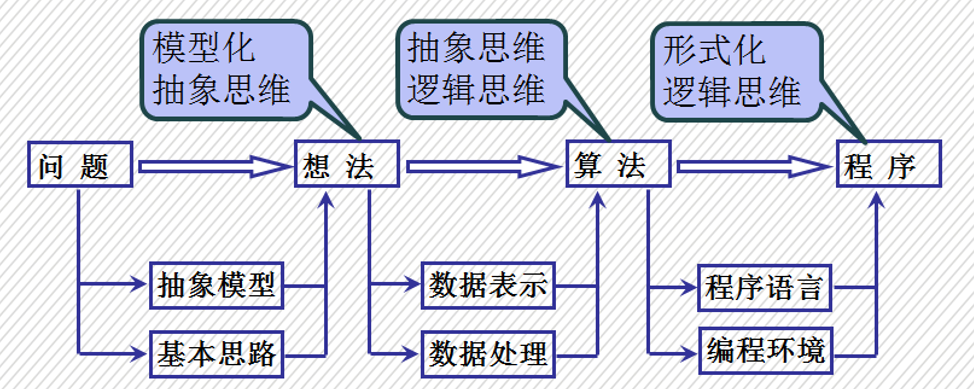
\includegraphics[width=.8\linewidth]{images/three_stages.png}
        \end{figure} 
      \end{minipage}\hfill
      \begin{minipage}{0.48\linewidth}
        \begin{enumerate}
            \item 界定与分析问题
            \item 建模
            \item 选择解决方法
            \item 设计处理算法
            \item 程序化
            \item 算法分析
          \end{enumerate}
      \end{minipage}
\end{frame}


\begin{frame}
\frametitle{程序的控制结构}
结构化的程序设计就是把一个程序分成若干互相独立的模块。基本要点：
\begin{enumerate}
  \item 自上而下，逐步细化
  
  将复杂的大问题逐步分解多个简单的小问题。
  \item 模块化设计
  
  一个程序是由一个主控模块和若干个子模块组成的。
  \item 结构化编码
\end{enumerate}
\begin{center}
  \begin{tikzpicture}[semithick,draw=DeepSkyBlue2,node distance=1.5cm,scale=0.9,every node/.style={scale=0.9}]
    \node (A1) [startstop] {主控模块};
    \node (B2) [startstop, below of=A1] {子模块2};
    \node (B1) [startstop, below of=A1,xshift=-4cm] {子模块1};
    \node (B3) [startstop, below of=A1,xshift=4cm] {子模块3};
    \node (C22) [startstop, below of=B2,xshift=2cm] {子模块22};
    \node (C23) [startstop, right of=C22,xshift=1cm] {子模块23};
    \node (C21) [startstop, left of=C22,xshift=-1cm] {子模块21};
    \node (C12) [startstop, left of=C21,xshift=-1cm] {子模块12};
    \node (C11) [startstop, left of=C12,xshift=-1cm] {子模块11};
    \draw [->] (A1) -- (B2);
    \draw [->] (A1) --++ (0,-0.7) -| (B1);
    \draw [->] (A1) --++ (0,-0.7) -| (B3);
    \draw [->] (B1) --++ (0,-0.7) -| (C11);
    \draw [->] (B1) --++ (0,-0.7) -| (C12);
    \draw [->] (B2) --++ (0,-0.7) -| (C21);
    \draw [->] (B2) --++ (0,-0.7) -| (C22);
    \draw [->] (B2) --++ (0,-0.7) -| (C23);
\end{tikzpicture}
\end{center}  
\end{frame}


\begin{frame}
  \frametitle{编程语言}
    \begin{minipage}{0.28\linewidth}
      和人沟通：
      \begin{itemize}
        \item 汉语
        \item 英语
        \item $\cdots \cdots$
      \end{itemize}
    
      和计算机沟通：
      \begin{itemize}
        \item C
        \item python
        \item java
        \item $\cdots \cdots$
      \end{itemize}
      \end{minipage}\hfill
      \begin{minipage}{0.68\linewidth}
        \begin{figure}[htpb]
          \centering
          
\includegraphics[width=.9\linewidth]{images/languages.jpg}
        \end{figure} 
      \end{minipage}
  
\end{frame}

\begin{frame}
    \frametitle{编程语言流行度 \link{https://www.tiobe.com/tiobe-index/}}
    \vspace{-1em}
    \begin{figure}[htpb]
        \centering
        \caption{TIOBE Index for November 2023}
        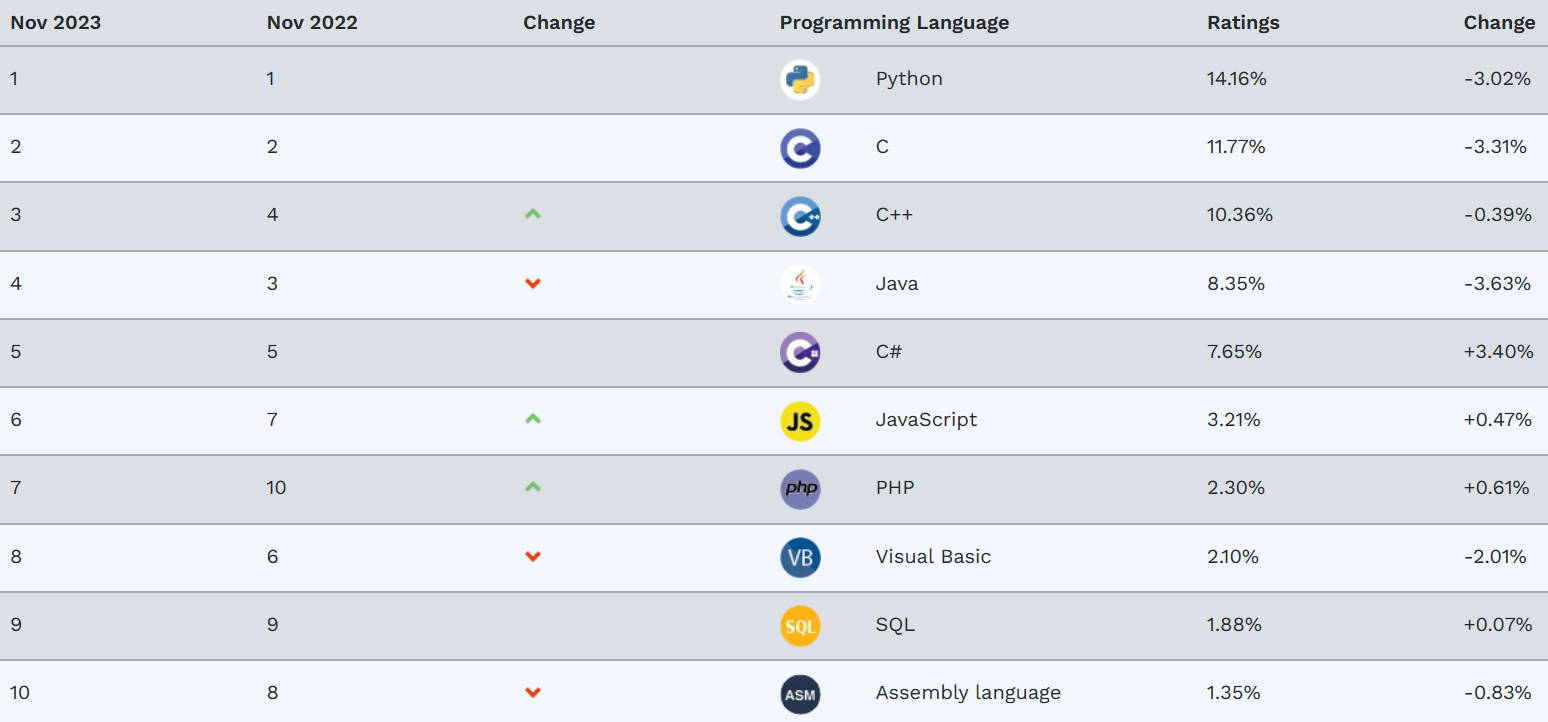
\includegraphics[width=.85\linewidth]{images/TIOBE Index}
    \end{figure}
\end{frame}

\begin{frame}
    \frametitle{计算机二级}
    \begin{multicols}{2}
        \begin{itemize}
            \item C语言程序设计
            \item Java语言程序设计
            \item C++语言程序设计
            \item Python语言程序设计
            \item Web程序设计
            \item MS Office高级应用与设计
            \item WPS Office高级应用与设计
            \item Access数据库程序设计
            \item MySQL数据库程序设计
            \item openGauss数据库程序设计
        \end{itemize}
    \end{multicols}
\end{frame}

\begin{frame}
    \frametitle{编程语言对比}
\begin{table}[]
    \begin{tabular}{@{}cccc@{}}
    \toprule
                    & \textbf{优点}                                                   & \textbf{缺点}                                                      & \textbf{典型应用领域}                                                    \\ \midrule
    \textbf{Python} & \begin{tabular}[c]{@{}c@{}}易于学习\\      丰富的库\end{tabular}      & \begin{tabular}[c]{@{}c@{}}运行速度较慢\\      内存占用较大\end{tabular}     & \begin{tabular}[c]{@{}c@{}}科学计算和数据分析\\      机器学习和人工智能\end{tabular} \\ \midrule
    \textbf{C}      & \begin{tabular}[c]{@{}c@{}}运行速度快\\      跨平台性非常好\end{tabular}  & \begin{tabular}[c]{@{}c@{}}复杂的学习曲线\\      不支持面向对象编程\end{tabular} & \begin{tabular}[c]{@{}c@{}}操作系统开发\\      嵌入式系统\end{tabular}        \\ \midrule
    \textbf{Java}   & \begin{tabular}[c]{@{}c@{}}自动管理内存\\      跨平台性非常好\end{tabular} & \begin{tabular}[c]{@{}c@{}}占用大量内存\\      启动时间较长\end{tabular}     & \begin{tabular}[c]{@{}c@{}}Web编程\\      应用程序开发\end{tabular}        \\ \midrule
    \textbf{C++}    & \begin{tabular}[c]{@{}c@{}}性能高\\      可以直接访问硬件\end{tabular}   & \begin{tabular}[c]{@{}c@{}}学习曲线陡峭\\      代码可读性差\end{tabular}     & \begin{tabular}[c]{@{}c@{}}游戏开发\\      操作系统和驱动程序\end{tabular}      \\ \bottomrule
    \end{tabular}
    \end{table}
\end{frame}


\begin{frame}
    \frametitle{学习程序设计的好处}
    \begin{enumerate}
      \item 计算机已经成为我们生活、学习和工作中普遍使用的工具，学会编程能使我们解决很多问题。
      \item 程序设计能够培养我们抽象、分析和问题求解的能力，这种能力对日常生活和工作也是很重要的。
      \item 编程也是一种充满乐趣的智力活动，许多人将编程当作一种爱好，发现巧妙的算法和程序运行成功后的那种成就感令人乐此不疲。
    \end{enumerate}
\end{frame}


\begin{frame}[fragile]
    \frametitle{}
\begin{codeblock}[firstline=1, lastline =15]{随机点名程序}
  import random
  import tkinter as tk
  
  
  class RollCallApp:
      def __init__(self, students):
          self.students = students
          self.roll_call_running = False
  
          self.window = tk.Tk()
          self.window.title("班级点名程序")
          self.window.geometry("400x200")
  
          self.student_name = tk.StringVar()
          self.student_name.set("请开始点名")
  
          self.label = tk.Label(self.window, textvariable=self.student_name, font=("微软雅黑", 24), fg="red")
          self.label.pack(pady=20)
  
          self.button = tk.Button(self.window, text="开始点名", font=("微软雅黑", 16),  command=self.roll_call)
          self.button.pack(pady=10)
  
      def roll_call(self):
          if not self.roll_call_running:
              self.roll_call_running = True
              self.button.config(text="停止滚动")
              self.roll_call_loop()
          else:
              self.roll_call_running = False
              self.button.config(text="开始点名")
  
      def roll_call_loop(self):
          student = random.choice(self.students)
          self.student_name.set(student)
  
          if self.roll_call_running:
              self.window.after(100, self.roll_call_loop)
  
      def run(self):
          self.window.mainloop()
  
  
  students = ["Alice", "Bob", "Charlie", "David", "Emily", "Frank", "Grace", "Harry", "Isabella", "Jack", "Kevin", "Lily", "Maggie", "Nancy", "Oliver", "Peter"]
  
  app = RollCallApp(students)
  app.run()
\end{codeblock}
\end{frame}

\begin{frame}[fragile]  
  \frametitle{}  
\begin{codeblock}[firstline=16, lastline =30, firstnumber=16]{}
  import random
  import tkinter as tk
  
  
  class RollCallApp:
      def __init__(self, students):
          self.students = students
          self.roll_call_running = False
  
          self.window = tk.Tk()
          self.window.title("班级点名程序")
          self.window.geometry("400x200")
  
          self.student_name = tk.StringVar()
          self.student_name.set("请开始点名")
  
          self.label = tk.Label(self.window, textvariable=self.student_name, font=("微软雅黑", 24), fg="red")
          self.label.pack(pady=20)
  
          self.button = tk.Button(self.window, text="开始点名", font=("微软雅黑", 16),  command=self.roll_call)
          self.button.pack(pady=10)
  
      def roll_call(self):
          if not self.roll_call_running:
              self.roll_call_running = True
              self.button.config(text="停止滚动")
              self.roll_call_loop()
          else:
              self.roll_call_running = False
              self.button.config(text="开始点名")
  
      def roll_call_loop(self):
          student = random.choice(self.students)
          self.student_name.set(student)
  
          if self.roll_call_running:
              self.window.after(100, self.roll_call_loop)
  
      def run(self):
          self.window.mainloop()
  
  
  students = ["Alice", "Bob", "Charlie", "David", "Emily", "Frank", "Grace", "Harry", "Isabella", "Jack", "Kevin", "Lily", "Maggie", "Nancy", "Oliver", "Peter"]
  
  app = RollCallApp(students)
  app.run()

\end{codeblock}
\end{frame}


\begin{frame}[fragile]  
  \frametitle{}  
\begin{codeblock}[firstline=31, lastline =50, firstnumber=31]{}
  import random
  import tkinter as tk
  
  
  class RollCallApp:
      def __init__(self, students):
          self.students = students
          self.roll_call_running = False
  
          self.window = tk.Tk()
          self.window.title("班级点名程序")
          self.window.geometry("400x200")
  
          self.student_name = tk.StringVar()
          self.student_name.set("请开始点名")
  
          self.label = tk.Label(self.window, textvariable=self.student_name, font=("微软雅黑", 24), fg="red")
          self.label.pack(pady=20)
  
          self.button = tk.Button(self.window, text="开始点名", font=("微软雅黑", 16),  command=self.roll_call)
          self.button.pack(pady=10)
  
      def roll_call(self):
          if not self.roll_call_running:
              self.roll_call_running = True
              self.button.config(text="停止滚动")
              self.roll_call_loop()
          else:
              self.roll_call_running = False
              self.button.config(text="开始点名")
  
      def roll_call_loop(self):
          student = random.choice(self.students)
          self.student_name.set(student)
  
          if self.roll_call_running:
              self.window.after(100, self.roll_call_loop)
  
      def run(self):
          self.window.mainloop()
  
  
  students = ["Alice", "Bob", "Charlie", "David", "Emily", "Frank", "Grace", "Harry", "Isabella", "Jack", "Kevin", "Lily", "Maggie", "Nancy", "Oliver", "Peter"]
  
  app = RollCallApp(students)
  app.run()

\end{codeblock}
\end{frame}




\subsection{算法的评价}

\begin{frame}
    \frametitle{算法的评价}
    解决某一问题存在多种算法，为了有效地进行解题，不仅需要保证算法正确，还要考虑算法的质量，那怎样才算是一个优秀的算法呢？一般有这么几个标准：

  （1）正确性（2）可读性（3）健壮性（4）效率
  \bigskip

  \begin{block}{以效率为标准举例：称金币问题}
    9个外观一样的金币，其中一个赝品重量较轻。如果用天平秤鉴别真伪，至少需要称几次才能保证找出假币？
  \end{block}
    \pause

    算法1：天平左边金币固定，不断变换右边金币，最多称7次可鉴别出假币。

    算法2：天平两边各一个金币，每次变换两边金币，最多称4次可鉴别出假币。

    算法3：天平左边3个，右边3个，留下3个，最多称2次可以鉴别出假币。

\end{frame}

\begin{frame}
    \frametitle{算法复杂度}
    为了更公平的比较和衡量算法质量的优劣程序，需要一个客观的标准，这个标准就是著名计算机科学家，算法分析之父高德纳提出的 {\cbf{算法复杂度}}。
    \begin{itemize}
      \item {\cbf{时间复杂度}}
      
      有许多因素可能会影响算法在特定计算机上的运行时间，因此，大 O 表示法不关注算法运行的实际时间，而是根据需要执行的操作数量来定义运行时间。
      \item {\cbf{空间复杂度}}
      
      该算法所耗费的存储空间

      在平时的开发中更多的是用空间换时间
    \end{itemize}
\end{frame}

\begin{frame}
    \frametitle{常见时间复杂度}
    \begin{columns}
      \begin{column}{.45\textwidth}
        \begin{table}
          \centering
          \begin{tabular}{lc}
            \toprule
            \cbf{大O记法} & \cbf{非正式术语} \\ \midrule
            O($n^2$) & 平方阶 \\
            O($n\log n$) & 线性对数阶 \\
            O($n$) & 线性阶 \\
            O($\log n$) & 对数阶 \\
            O(1) & 常数阶 \\ \bottomrule
          \end{tabular}
        \end{table}
      \end{column}\hfill
      \begin{column}{.5\textwidth}
        \begin{center}
          \begin{tikzpicture}[thick,scale=0.55]
            \draw[->] (-0.2,0) --(10,0) node[right] {$n$};
            \draw[->] (0,-0.2) --(0,10) node[above] {$T(n)$};
            \draw[domain =0:3,Tomato1] plot (\x ,{(\x)^2}) node[right] {O($n^2$)};
            \draw[RoyalBlue1] plot [domain=1:4,samples=100] (\x,{\x*log2(\x)}) node[right] {O($n \log n$)};
            \draw[domain =0:9,PaleVioletRed1] plot (\x ,\x) node[right] {O($n$)};
            \draw[Cyan4] plot [domain=1:9,samples=100] (\x,{log2(\x)}) node[right] {O($\log n$)};
            \draw[Red1] (0,0) -- (9,0) node[above,near end] {O(1)};
            \foreach \x in {0,1,2,3,4,5,6,7,8,9}
            \draw (\x,0) -- (\x,-0.2) node [below] {\x};
        \end{tikzpicture}
        \end{center}
      \end{column}
    \end{columns}
\end{frame}

% 计算机科学中log默认以2为底

